%%%%%%%%%%%%%%%%%%%%%%%%%%%%%%% main.tex %%%%%%%%%%%%%%%%%%%%%%%%%%%%%%%
%                                                                      %
% --------------------- Report Template IST [EN] --------------------- %
%                                                                      %
%       João Marafuz Gaspar                                            %
%       Departamento de Engenharia Eletrotécnica e de Computadores     %
%       Instituto Superior Tecnico                                     %
%       Av. Rovisco Pais                                               %
%       1049-001 Lisboa                                                %
%       Portugal                                                       %
%       E-mail: joao.marafuz.gaspar@tecnico.ulisboa.pt                 %
%                                                                      %
%  Created:       Jul 30, 2022                                         %
%  Last Modified: Apr 6, 2023                                          %
%                                                                      %
%%%%%%%%%%%%%%%%%%%%%%%%%%%%%%%%%%%%%%%%%%%%%%%%%%%%%%%%%%%%%%%%%%%%%%%%
%  Revision history                                                    %
%  v1 - 2022/07/30 - original template                                 %
%  v2 - 2023/04/06 - change superscript in the cover, updated font,    %
%                    added subfigures and table                        %
%%%%%%%%%%%%%%%%%%%%%%%%%%%%%%%%%%%%%%%%%%%%%%%%%%%%%%%%%%%%%%%%%%%%%%%%
%                              Preamble                                %
%%%%%%%%%%%%%%%%%%%%%%%%%%%%%%%%%%%%%%%%%%%%%%%%%%%%%%%%%%%%%%%%%%%%%%%%

% ----------------------------------------------------------------------
% Set the document class
% ----------------------------------------------------------------------
\documentclass[12pt]{article}

% ----------------------------------------------------------------------
% Define external packages, language, margins, fonts, new commands 
% and colors
% ----------------------------------------------------------------------
\usepackage[utf8]{inputenc} % Codification
\usepackage[english]{babel} % Writing idiom

\usepackage[export]{adjustbox} % Align images
\usepackage{amsmath} % Extra commands for math mode
\usepackage{amssymb} % Mathematical symbols
\usepackage{anysize} % Personalize margins
    \marginsize{2cm}{2cm}{2cm}{2cm} % {left}{right}{above}{below}
\usepackage{appendix} % Appendices
\usepackage{cancel} % Expression cancellation
\usepackage{caption} % Captions
    \DeclareCaptionFont{newfont}{\fontfamily{cmss}\selectfont}
    \captionsetup{labelfont={bf, newfont}}
\usepackage{cite} % Citations, like [1 - 3]
\usepackage{color} % Text coloring
\usepackage{fancyhdr} % Head note and footnote
    \pagestyle{fancy}
    \fancyhf{}
    \fancyhead[L]{\footnotesize \fontfamily{cmss}\selectfont IUST} % Left of Head note
    \fancyhead[R]{\footnotesize \fontfamily{cmss}\selectfont News Classification} % Right of Head note
    \fancyfoot[L]{\footnotesize \fontfamily{cmss}\selectfont Natural Language Processing} % Left of Footnote
    \fancyfoot[C]{\thepage} % Center of Footnote
    \renewcommand{\footrulewidth}{0.4pt} % Footnote rule
\usepackage{float} % Utilization of [H] in figures
\usepackage{graphicx} % Figures in LaTeX
\usepackage[colorlinks = true, plainpages = true, linkcolor = istblue, urlcolor = istblue, citecolor = istblue, anchorcolor = istblue]{hyperref}
\usepackage{indentfirst} % First paragraph
\usepackage[super]{nth} % Superscripts
\usepackage{siunitx} % SI units
\usepackage{subcaption} % Subfigures
\usepackage{titlesec} % Font
    \titleformat{\section}{\fontfamily{cmss}\selectfont\Large\bfseries}{\thesection}{1em}{}
    \titleformat{\subsection}{\fontfamily{cmss}\selectfont\large\bfseries}{\thesubsection}{1em}{}
    \titleformat{\subsubsection}{\fontfamily{cmss}\selectfont\normalsize\bfseries}{\thesubsubsection}{1em}{}
    \fancyfoot[C]{\fontfamily{cmss}\selectfont\thepage}

% Random text (not needed)
\usepackage{lipsum}
\usepackage{duckuments}
\usepackage{tikz}
\usetikzlibrary{calc}
\usepackage{eso-pic}

\usepackage{lipsum}

\AddToShipoutPictureBG{%
\begin{tikzpicture}[overlay,remember picture]
\draw[line width=4pt]
    ($ (current page.north west) + (1cm,-1cm) $)
    rectangle
    ($ (current page.south east) + (-1cm,1cm) $);
\draw[line width=1.5pt]
    ($ (current page.north west) + (1.2cm,-1.2cm) $)
    rectangle
    ($ (current page.south east) + (-1.2cm,1.2cm) $);
\end{tikzpicture}
}

\usepackage{hyperref}
\usepackage{csvsimple}

% New and re-newcommands
\newcommand{\sen}{\operatorname{\sen}} % Sine function definition
\newcommand{\HRule}{\rule{\linewidth}{0.5mm}} % Specific rule definition
\renewcommand{\appendixpagename}{\LARGE \fontfamily{cmss}\selectfont Appendices}

% Colors
\definecolor{istblue}{RGB}{3, 171, 230}
\definecolor{dkgreen}{rgb}{0,0.6,0}
\definecolor{gray}{rgb}{0.5,0.5,0.5}

%%%%%%%%%%%%%%%%%%%%%%%%%%%%%%%%%%%%%%%%%%%%%%%%%%%%%%%%%%%%%%%%%%%%%%%%
%                                 Document                             %
%%%%%%%%%%%%%%%%%%%%%%%%%%%%%%%%%%%%%%%%%%%%%%%%%%%%%%%%%%%%%%%%%%%%%%%%
\begin{document}

% ----------------------------------------------------------------------
% Cover
% ----------------------------------------------------------------------
\begin{center}
    \begin{figure}
        \vspace{-1.0cm}
        
\includegraphics[scale = 0.3, left]{Images/IUSTLogo.png} % IST logo
    \end{figure}
    \mbox{}\\[2.0cm]
    \textsc{\Huge Natural Language Processing}\\[2.5cm]
    \textsc{\LARGE Supervisor: Dr. Seyed Saleh Etemadi}\\[2.0cm]
    \HRule\\[0.4cm]
    {\large \bf {\fontfamily{cmss}\selectfont News Classification}}\\[0.2cm]
    \HRule\\[1.5cm]
\end{center}

\begin{flushleft}
    \textbf{\fontfamily{cmss}\selectfont Author:}
\end{flushleft}

\begin{center}
    \begin{minipage}{0.5\textwidth}
        \begin{flushleft}
            Elnaz Rezaee
        \end{flushleft}
    \end{minipage}%
    \begin{minipage}{0.5\textwidth}
        \begin{flushright}
            \href{mailto:joao.marafuz.gaspar@tecnico.ulisboa.pt}{\texttt{elnazrezaee80@gmail.com}}
        \end{flushright}
    \end{minipage}
\end{center}
    
\begin{center}
    \large \bf \fontfamily{cmss}\selectfont 2023/2024
\end{center}

\thispagestyle{empty}

\setcounter{page}{0}

\newpage

% ----------------------------------------------------------------------
% Contents
% ----------------------------------------------------------------------
\tableofcontents 

\newpage

% ----------------------------------------------------------------------
% Body
% ----------------------------------------------------------------------
\section{Introduction}

The purpose of this project is to analyze and process fact-checking data obtained from Politifact. The data consists of statements from different categories, including "true," "mostly true," "half true," "barely true," "false," and "pants on fire." The data was collected by scraping the Politifact website and subsequently cleaned and preprocessed for further analysis.

\section{Accurate data source} 

The data source of this project is the \href{https://www.politifact.com/factchecks/list}{\textcolor{istblue}{PolitiFact}} website, which categorizes the data into 6 classes with the titles stated in the introduction section. Also, for the data to be balanced, a specific number (2500) of data has been collected from each category.

\section{Data collection methodology}

The data collection for this report involved a systematic approach utilizing various steps and tools. The following outlines the methodology employed:

\begin{itemize}
  \item \textbf{Selection of data sources}: The data for this report was collected from Politifact, a reputable fact-checking organization known for its unbiased analysis of statements made by politicians and public figures. Politifact provides a comprehensive repository of fact-checks, ratings, and statements, making it an ideal source for this research.
  
  \item \textbf{Web scraping}: The data was collected from the Politifact website using web scraping techniques. The \texttt{BeautifulSoup} library in Python was utilized to extract information from the HTML pages. The \texttt{requests} library facilitated the HTTP requests to retrieve the web pages.
  
  \item \textbf{Data Cleaning}: The collected data underwent a cleaning process to remove any irrelevant or noisy information. The \texttt{pandas} library was used to read the raw data, and cleaning operations were performed to ensure consistency and accuracy.
  
  \item \textbf{Text Processing}: To analyze the textual content of the statements, various text processing techniques were applied. The \texttt{nltk} library was employed to tokenize the statements into sentences, while the \texttt{spacy} library facilitated the tokenization of words for further analysis.
\end{itemize}

These steps were carried out using the Python programming language and various libraries such as \texttt{csv}, \texttt{json}, and \texttt{urllib3}. The collected data was stored in CSV format for easy accessibility and further analysis.

By following this robust data collection methodology and utilizing appropriate tools, the integrity and accuracy of the data used in this report were ensured.

\section{Data format}

The collected data is organized in a specific file and folder structure to ensure efficient storage and retrieval. The following outlines the structure of each file and provides an explanation of the different tags:

\subsection{File Structure}

The data is stored in CSV (Comma-Separated Values) format, which is a widely used format for tabular data. The data folder, contains 4 categories including raw, clean, sentencebroken and wordbroken. Each of these folders, have 6 CSV files as follows: 

\begin{verbatim}
- true.csv
- mostly-true.csv
- half-true.csv
- barely-true.csv
- false.csv
- pants-fire.csv
\end{verbatim}

Each CSV file corresponds to a specific truthfulness category and contains two columns: \texttt{Statement} and \texttt{Label}. The \texttt{Statement} column stores the fact-check statements, while the \texttt{Label} column represents the truthfulness rating associated with each statement.

\subsection{Differentiation of Tags}

The data collected from Politifact utilizes different tags to represent the truthfulness rating of each statement. The tags used and their meanings are as follows:

\begin{itemize}
  \item \textbf{True}: This tag represents statements that have been fact-checked and determined to be completely accurate and truthful.
  
  \item \textbf{Mostly True}: Statements labeled as "Mostly True" indicate that they contain some degree of truth but may also include some inaccuracies or misleading information.
  
  \item \textbf{Half True}: This tag is assigned to statements that are partially true but also contain some false or misleading elements.
  
  \item \textbf{Barely True}: Statements labeled as "Barely True" are mostly false but may contain a small element of truth.
  
  \item \textbf{False}: This tag represents statements that have been fact-checked and determined to be false or misleading.
  
  \item \textbf{Pants on Fire}: The "Pants on Fire" tag is used for statements that are blatantly false or entirely fabricated.
\end{itemize}

By categorizing the statements into different tags based on their truthfulness, the data allows for further analysis and evaluation of the reliability and accuracy of the statements made by politicians and public figures.

\section{Pre-processing}

The following pre-processing steps were performed:

\subsection{Sentence separation}
Sentences were separated using the nltk library. So, the method of sentence breaking is performed using the $nltk.sent\_tokenize()$ function.

\subsection{Tokens/Words separation}
Tokens/words were separated using the spaCy library. The statement is passed through the spaCy pipeline to obtain a processed document object (doc). The tokens in the document object are extracted and stored as a list of strings. So, the text is splitted by words.

\subsection{Data cleaning}
 The data was cleaned using the implemented data cleaning method. The \texttt{clean\_data} function takes a \texttt{text} parameter, which represents the input text that needs to be cleaned.

Within the function, the \texttt{re.sub()} method is used to perform regular expression-based substitution in the text. The regular expression pattern \texttt{r'[\^{}a-zA-Z0-9. \$]'} matches any character that is not an alphabet letter (lowercase or uppercase), a digit, a period, a space, or a dollar sign.

The \texttt{re.sub()} method replaces all occurrences of the matched pattern with an empty string, effectively removing them from the text. This helps in eliminating unwanted characters or symbols from the text. The cleaned text is then returned from the function.

\subsection{Data size Before/After Cleaning}

The data size before and after cleaning is as follows:

\begin{itemize}
  \item Data Size Before Cleaning: 1878218 bytes
  \item Data Size After Cleaning: 1770027 bytes
\end{itemize}

\section{Tagging unit and tagging method}

The tagging unit in this project claims from the Politifact dataset.The labels represent different categories such as "true", "mostly-true", "half-true", "barely-true", "false", and "pants-fire".

The tagging method is based on the labels provided by Politifact, which are assigned to the statements based on their assessment of truthfulness. Each statement is associated with a specific label that indicates its categorization or classification.

The tagging process involves extracting the statements from the dataset and assigning the corresponding label to each statement. This is done by parsing the HTML content of the Politifact website, retrieving the statement and label information, and storing them in separate CSV files.

\section{Data statistics}
\subsection{Number of units of data}
\begin{align*}
    \csvautotabular{CSVs/data-counts.csv}
\end{align*}

\subsection{Number of sentences}
\begin{align*}
    \csvautotabular{CSVs/sentence-counts.csv}
\end{align*}

\subsection{Number of words}
\begin{align*}
    \csvautotabular{CSVs/word-counts.csv}
\end{align*}

\subsection{Unique word count}
\begin{align*}
    \csvautotabular{CSVs/unique-word-counts.csv}
\end{align*}

\subsection{Number of unique words common and uncommon between labels}
\begin{align*}
    \csvautotabular{CSVs/common-uncommon-counts.csv}
\end{align*}

\subsection{10 most frequent non-shared words from each label}
\begin{align*}
    \csvautotabular{CSVs/most-frequent-uncommon-words.csv}
\end{align*}

\subsection{Top 10 common words of each label compared to other labels based on relative frequency}
\begin{align*}
    \csvautotabular{CSVs/top-relative-frequency-words.csv}
\end{align*}

\subsection{Top 10 words of each label based on TF-IDF($w_i$)}
\begin{align*}
    \csvautotabular{CSVs/top-tf-idf-words.csv}
\end{align*}

\subsection{Histogram of the number of repetitions of each unique word}

\begin{figure}[H]
	\begin{center}
 		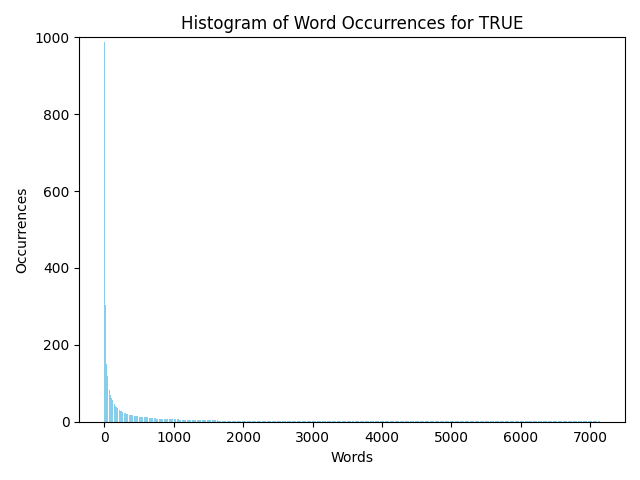
\includegraphics[width = 0.7\textwidth]{Images/true-histogram.png}
 		\caption{Histogram of label "True"}
 		\label{fig:1}
	\end{center} 
\end{figure}

\begin{figure}[H]
	\begin{center}
 		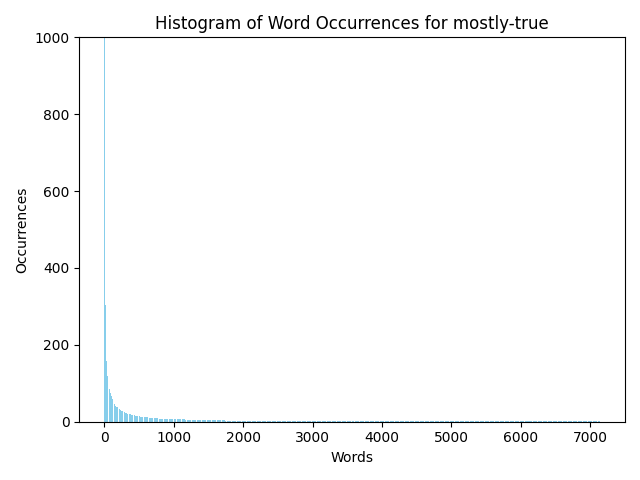
\includegraphics[width = 0.7\textwidth]{Images/mostly-true-histogram.png}
 		\caption{Histogram of label "Mostly True"}
 		\label{fig:1}
	\end{center} 
\end{figure}

\begin{figure}[H]
	\begin{center}
 		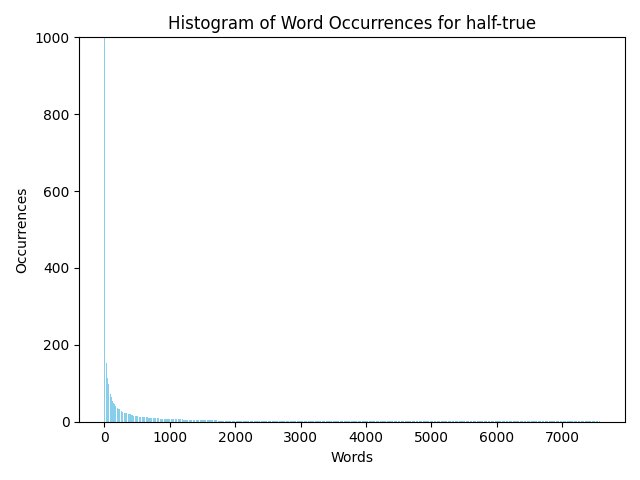
\includegraphics[width = 0.7\textwidth]{Images/half-true-histogram.png}
 		\caption{Histogram of label "Half True"}
 		\label{fig:1}
	\end{center} 
\end{figure}

\begin{figure}[H]
	\begin{center}
 		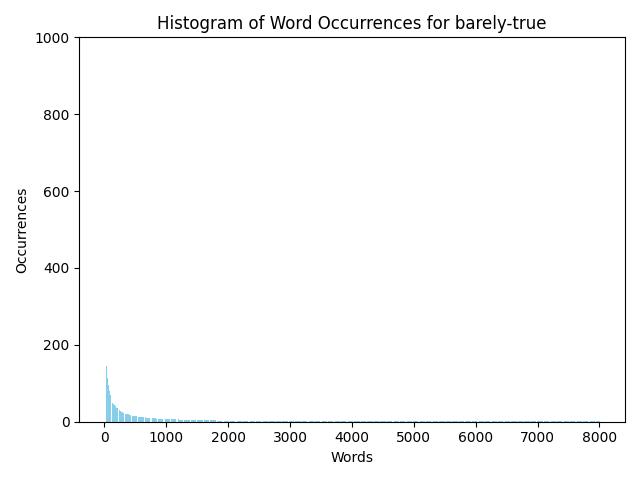
\includegraphics[width = 0.7\textwidth]{Images/barely-true-histogram.png}
 		\caption{Histogram of label "Barely True"}
 		\label{fig:1}
	\end{center} 
\end{figure}

\begin{figure}[H]
	\begin{center}
 		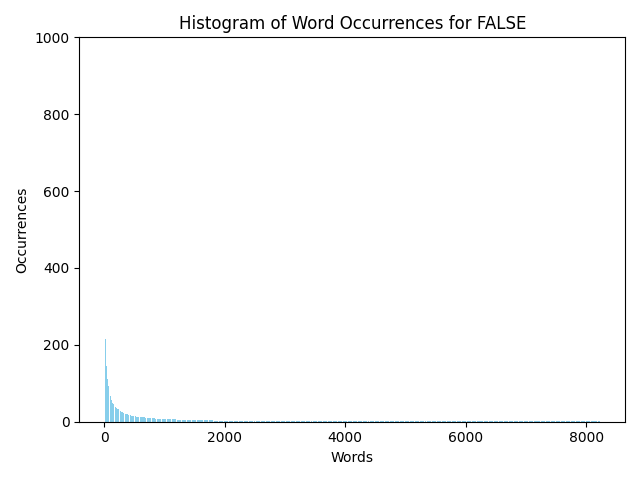
\includegraphics[width = 0.7\textwidth]{Images/false-histogram.png}
 		\caption{Histogram of label "False"}
 		\label{fig:1}
	\end{center} 
\end{figure}

\begin{figure}[H]
	\begin{center}
 		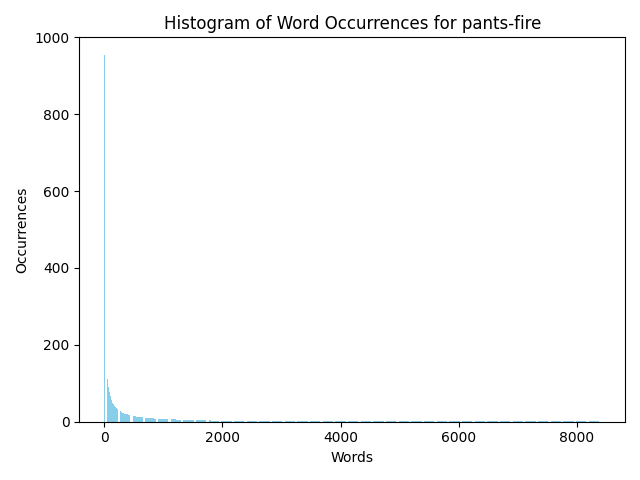
\includegraphics[width = 0.7\textwidth]{Images/pants-fire-histogram.png}
 		\caption{Histogram of label "Pants on Fire"}
 		\label{fig:1}
	\end{center} 
\end{figure}

\href{https://github.com/lelnazrezaeel/News-Classification/tree/main}{\textcolor{istblue}{Click here to see my github.}}

\href{https://huggingface.co/datasets/elnazrezaee/News-Classification-Dataset/tree/main}{\textcolor{istblue}{Click here to see my dataset.}}
\end{document}